\documentclass{article}

\usepackage[final]{nips_2018}

% to avoid loading the natbib package, add option nonatbib:
% \usepackage[nonatbib]{nips_2018}

\usepackage[utf8]{inputenc} % allow utf-8 input
\usepackage[T1]{fontenc}    % use 8-bit T1 fonts
\usepackage{hyperref}       % hyperlinks
\usepackage{url}            % simple URL typesetting
\usepackage{booktabs}       % professional-quality tables
\usepackage{amsfonts}       % blackboard math symbols
\usepackage{nicefrac}       % compact symbols for 1/2, etc.
\usepackage{microtype}      % microtypography

\usepackage{graphicx}
\usepackage{cite}

\title{BLACK: Body Language Affect Classification Kernel}

\author{
  Undergrad-ient Descent Expedition: \\
  Jack (Xiang) Zhou, Karan Aujla, James Bie, Eric Gao, Insoo Rhee\\
  Faculty of Applied Sciences\\
  Simon Fraser University\\
  Burnaby, Canada\\
  \texttt{xza194@sfu.ca} \\
}

\begin{document}

\maketitle

\begin{abstract}
  This is the abstract of the paper that we are going to write
\end{abstract}

\section{Introduction}
% cite BEAST
% cite COBOL
awooo 56709

Talk about COBOL, work has been done before but not on a skeleton level
\section{Approach}
\subsection{Architecture}

We introduce the general architecture of the overall pipeline in this section. The novel and primary goal of the present work is to assign affective labels with learned patterns in body langauge. However, as we are only in the primary stage in this pursuit and we do not have a comprehensive method toward accounting for viewpoint invariance, using body posture as the primary is not very realistic. In the present work we use body language mainly as a supplement to existing facial affective labels if it is detected.

A snapshot is taken from an arbitrary visual stream and the resulting image is passed into OpenPose to detect all persons. For each person: (1) If a face was found, then it is passed into a face-based classifier for an evaluation of the affective rating vector based solely on face. (2) If a body was found, then it is passed into a body language-based classifier for an evaluation of the affective rating vector based solely on body. A weighted sum is computed between (1) and (2) for each person. If only one of (1) or (2) is found, then only that one is taken. A grand total is calculated by summing over every person's weighted sum of affective labels. The grand total will be passed into a softmax function to obtain a probability vector of the model prediction. A graphical depiction of this overall process is shown in Figure 1.

\begin{figure}[h]
	\centering
	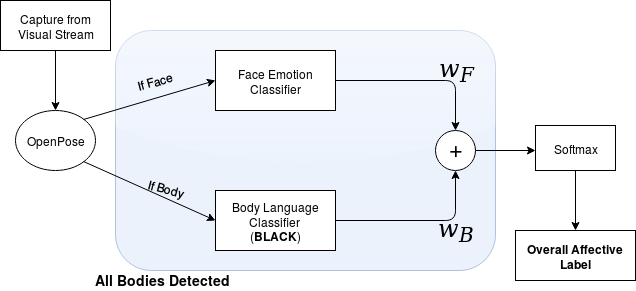
\includegraphics[scale=0.5]{Pipeline}
	\caption{The overall pipeline.}
\end{figure}

\subsubsection{Body Language Keypoint Estimation}

To extract body keypoints, we used the OpenPose system produced by the CMU Perceptual Computing Laboratory ~\citep{cao2017realtime} ~\citep{simon2017hand} ~\citep{wei2016cpm}

\subsubsection{Face Emotion Classification}
aaaaaaa
\subsection{Training}
As the problem that the present model is trying to solve involve uncensored face along with body posture, it is particularly difficult to obtain relevant published datasets that are labelled and publicly available. Past research in this field involved manual construction of data from actors (cite COBOL here).

To address this issue, we manually construct a dataset of unlabelled images of humans with visible face and body posture by using authors of this paper as actors as well as sources on the internet. The face and body are both clearly visible in the training images. The image will not be given a label when it is fed into the training pipeline in a pseudounsupervised learning paradigm. We describe the training pipeline as follows:

\begin{figure}[h]
	\centering
	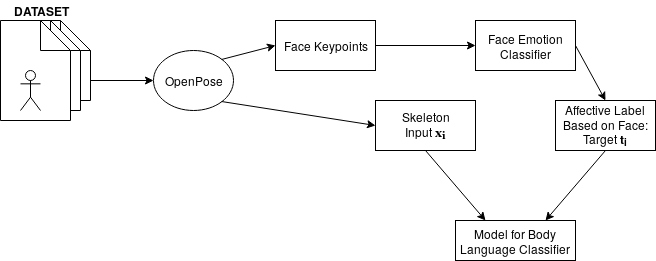
\includegraphics[scale=0.6]{tpipeline}
	\caption{The training pipeline.}
\end{figure}

The unlabelled image is first passed into OpenPose to obtain a set of posture keypoints (ie. a skeleton) of the human in the image, as well as a set of face keypoints. The face keypoints will be passed into an already trained face emotional classifier to give a ground truth affective label for the overall human in the image as informed by the face. The skeleton is then processed into an invariant form and used along with the affective label to train the body language affect classifier.

\section{Experiments}
\section{Conclusion}
\section{Contributions}

As with most group projects, each author of this paper contributed a considerable amount of work towards piecing together the project. Jack oversaw the project by organizing and delegating tasks for everyone as well as being the main composer of the paper and poster. Jack and James formulated the design of the overall pipeline for the models and for training the model. Karan worked with existing models for body posture keypoint extraction and implemented the top level program. Eric and James are the main contributors to data collection and piecing together a custom dataset for the project. Insoo and Jack worked on designing and implementing the model for mapping body keypoints to affective labels.

We would also like to thank Professor Angelica Lim for consultations and guidance toward the design and theoretical groundwork in the project.

%\section{Submission of papers to NIPS 2018}
%
%NIPS requires electronic submissions.  The electronic submission site
%is
%\begin{center}
%  \url{https://cmt.research.microsoft.com/NIPS2018/}
%\end{center}
%
%Please read the instructions below carefully and follow them faithfully.
%
%\subsection{Style}
%
%Papers to be submitted to NIPS 2018 must be prepared according to the
%instructions presented here. Papers may only be up to eight pages
%long, including figures. Additional pages \emph{containing only
%  acknowledgments and/or cited references} are allowed. Papers that
%exceed eight pages of content (ignoring references) will not be
%reviewed, or in any other way considered for presentation at the
%conference.
%
%The margins in 2018 are the same as since 2007, which allow for
%$\sim$$15\%$ more words in the paper compared to earlier years.
%
%Authors are required to use the NIPS \LaTeX{} style files obtainable
%at the NIPS website as indicated below. Please make sure you use the
%current files and not previous versions. Tweaking the style files may
%be grounds for rejection.
%
%\subsection{Retrieval of style files}
%
%The style files for NIPS and other conference information are
%available on the World Wide Web at
%\begin{center}
%  \url{http://www.nips.cc/}
%\end{center}
%The file \verb+nips_2018.pdf+ contains these instructions and
%illustrates the various formatting requirements your NIPS paper must
%satisfy.
%
%The only supported style file for NIPS 2018 is \verb+nips_2018.sty+,
%rewritten for \LaTeXe{}.  \textbf{Previous style files for \LaTeX{}
%  2.09, Microsoft Word, and RTF are no longer supported!}
%
%The \LaTeX{} style file contains three optional arguments: \verb+final+,
%which creates a camera-ready copy, \verb+preprint+, which creates a
%preprint for submission to, e.g., arXiv, and \verb+nonatbib+, which will
%not load the \verb+natbib+ package for you in case of package clash.
%
%\paragraph{New preprint option for 2018}
%If you wish to post a preprint of your work online, e.g., on arXiv,
%using the NIPS style, please use the \verb+preprint+ option. This will
%create a nonanonymized version of your work with the text
%``Preprint. Work in progress.''  in the footer. This version may be
%distributed as you see fit. Please \textbf{do not} use the
%\verb+final+ option, which should \textbf{only} be used for papers
%accepted to NIPS.
%
%At submission time, please omit the \verb+final+ and \verb+preprint+
%options. This will anonymize your submission and add line numbers to aid
%review. Please do \emph{not} refer to these line numbers in your paper
%as they will be removed during generation of camera-ready copies.
%
%The file \verb+nips_2018.tex+ may be used as a ``shell'' for writing
%your paper. All you have to do is replace the author, title, abstract,
%and text of the paper with your own.
%
%The formatting instructions contained in these style files are
%summarized in Sections \ref{gen_inst}, \ref{headings}, and
%\ref{others} below.
%
%\section{General formatting instructions}
%\label{gen_inst}
%
%The text must be confined within a rectangle 5.5~inches (33~picas)
%wide and 9~inches (54~picas) long. The left margin is 1.5~inch
%(9~picas).  Use 10~point type with a vertical spacing (leading) of
%11~points.  Times New Roman is the preferred typeface throughout, and
%will be selected for you by default.  Paragraphs are separated by
%\nicefrac{1}{2}~line space (5.5 points), with no indentation.
%
%The paper title should be 17~point, initial caps/lower case, bold,
%centered between two horizontal rules. The top rule should be 4~points
%thick and the bottom rule should be 1~point thick. Allow
%\nicefrac{1}{4}~inch space above and below the title to rules. All
%pages should start at 1~inch (6~picas) from the top of the page.
%
%For the final version, authors' names are set in boldface, and each
%name is centered above the corresponding address. The lead author's
%name is to be listed first (left-most), and the co-authors' names (if
%different address) are set to follow. If there is only one co-author,
%list both author and co-author side by side.
%
%Please pay special attention to the instructions in Section \ref{others}
%regarding figures, tables, acknowledgments, and references.
%
%\section{Headings: first level}
%\label{headings}
%
%All headings should be lower case (except for first word and proper
%nouns), flush left, and bold.
%
%First-level headings should be in 12-point type.
%
%\subsection{Headings: second level}
%
%Second-level headings should be in 10-point type.
%
%\subsubsection{Headings: third level}
%
%Third-level headings should be in 10-point type.
%
%\paragraph{Paragraphs}
%
%There is also a \verb+\paragraph+ command available, which sets the
%heading in bold, flush left, and inline with the text, with the
%heading followed by 1\,em of space.
%
%\section{Citations, figures, tables, references}
%\label{others}
%
%These instructions apply to everyone.
%
%\subsection{Citations within the text}
%
%The \verb+natbib+ package will be loaded for you by default.
%Citations may be author/year or numeric, as long as you maintain
%internal consistency.  As to the format of the references themselves,
%any style is acceptable as long as it is used consistently.
%
%The documentation for \verb+natbib+ may be found at
%\begin{center}
%  \url{http://mirrors.ctan.org/macros/latex/contrib/natbib/natnotes.pdf}
%\end{center}
%Of note is the command \verb+\citet+, which produces citations
%appropriate for use in inline text.  For example,
%\begin{verbatim}
%   \citet{hasselmo} investigated\dots
%\end{verbatim}
%produces
%\begin{quote}
%  Hasselmo, et al.\ (1995) investigated\dots
%\end{quote}
%
%If you wish to load the \verb+natbib+ package with options, you may
%add the following before loading the \verb+nips_2018+ package:
%\begin{verbatim}
%   \PassOptionsToPackage{options}{natbib}
%\end{verbatim}
%
%If \verb+natbib+ clashes with another package you load, you can add
%the optional argument \verb+nonatbib+ when loading the style file:
%\begin{verbatim}
%   \usepackage[nonatbib]{nips_2018}
%\end{verbatim}
%
%As submission is double blind, refer to your own published work in the
%third person. That is, use ``In the previous work of Jones et
%al.\ [4],'' not ``In our previous work [4].'' If you cite your other
%papers that are not widely available (e.g., a journal paper under
%review), use anonymous author names in the citation, e.g., an author
%of the form ``A.\ Anonymous.''
%
%\subsection{Footnotes}
%
%Footnotes should be used sparingly.  If you do require a footnote,
%indicate footnotes with a number\footnote{Sample of the first
%  footnote.} in the text. Place the footnotes at the bottom of the
%page on which they appear.  Precede the footnote with a horizontal
%rule of 2~inches (12~picas).
%
%Note that footnotes are properly typeset \emph{after} punctuation
%marks.\footnote{As in this example.}
%
%\subsection{Figures}
%
%\begin{figure}
%  \centering
%  \fbox{\rule[-.5cm]{0cm}{4cm} \rule[-.5cm]{4cm}{0cm}}
%  \caption{Sample figure caption.}
%\end{figure}
%
%All artwork must be neat, clean, and legible. Lines should be dark
%enough for purposes of reproduction. The figure number and caption
%always appear after the figure. Place one line space before the figure
%caption and one line space after the figure. The figure caption should
%be lower case (except for first word and proper nouns); figures are
%numbered consecutively.
%
%You may use color figures.  However, it is best for the figure
%captions and the paper body to be legible if the paper is printed in
%either black/white or in color.
%
%\subsection{Tables}
%
%All tables must be centered, neat, clean and legible.  The table
%number and title always appear before the table.  See
%Table~\ref{sample-table}.
%
%Place one line space before the table title, one line space after the
%table title, and one line space after the table. The table title must
%be lower case (except for first word and proper nouns); tables are
%numbered consecutively.
%
%Note that publication-quality tables \emph{do not contain vertical
%  rules.} We strongly suggest the use of the \verb+booktabs+ package,
%which allows for typesetting high-quality, professional tables:
%\begin{center}
%  \url{https://www.ctan.org/pkg/booktabs}
%\end{center}
%This package was used to typeset Table~\ref{sample-table}.
%
%\begin{table}
%  \caption{Sample table title}
%  \label{sample-table}
%  \centering
%  \begin{tabular}{lll}
%    \toprule
%    \multicolumn{2}{c}{Part}                   \\
%    \cmidrule(r){1-2}
%    Name     & Description     & Size ($\mu$m) \\
%    \midrule
%    Dendrite & Input terminal  & $\sim$100     \\
%    Axon     & Output terminal & $\sim$10      \\
%    Soma     & Cell body       & up to $10^6$  \\
%    \bottomrule
%  \end{tabular}
%\end{table}
%
%\section{Final instructions}
%
%Do not change any aspects of the formatting parameters in the style
%files.  In particular, do not modify the width or length of the
%rectangle the text should fit into, and do not change font sizes
%(except perhaps in the \textbf{References} section; see below). Please
%note that pages should be numbered.
%
%\section{Preparing PDF files}
%
%Please prepare submission files with paper size ``US Letter,'' and
%not, for example, ``A4.''
%
%Fonts were the main cause of problems in the past years. Your PDF file
%must only contain Type 1 or Embedded TrueType fonts. Here are a few
%instructions to achieve this.
%
%\begin{itemize}
%
%\item You should directly generate PDF files using \verb+pdflatex+.
%
%\item You can check which fonts a PDF files uses.  In Acrobat Reader,
%  select the menu Files$>$Document Properties$>$Fonts and select Show
%  All Fonts. You can also use the program \verb+pdffonts+ which comes
%  with \verb+xpdf+ and is available out-of-the-box on most Linux
%  machines.
%
%\item The IEEE has recommendations for generating PDF files whose
%  fonts are also acceptable for NIPS. Please see
%  \url{http://www.emfield.org/icuwb2010/downloads/IEEE-PDF-SpecV32.pdf}
%
%\item \verb+xfig+ "patterned" shapes are implemented with bitmap
%  fonts.  Use "solid" shapes instead.
%
%\item The \verb+\bbold+ package almost always uses bitmap fonts.  You
%  should use the equivalent AMS Fonts:
%\begin{verbatim}
%   \usepackage{amsfonts}
%\end{verbatim}
%followed by, e.g., \verb+\mathbb{R}+, \verb+\mathbb{N}+, or
%\verb+\mathbb{C}+ for $\mathbb{R}$, $\mathbb{N}$ or $\mathbb{C}$.  You
%can also use the following workaround for reals, natural and complex:
%\begin{verbatim}
%   \newcommand{\RR}{I\!\!R} %real numbers
%   \newcommand{\Nat}{I\!\!N} %natural numbers
%   \newcommand{\CC}{I\!\!\!\!C} %complex numbers
%\end{verbatim}
%Note that \verb+amsfonts+ is automatically loaded by the
%\verb+amssymb+ package.
%
%\end{itemize}
%
%If your file contains type 3 fonts or non embedded TrueType fonts, we
%will ask you to fix it.
%
%\subsection{Margins in \LaTeX{}}
%
%Most of the margin problems come from figures positioned by hand using
%\verb+\special+ or other commands. We suggest using the command
%\verb+\includegraphics+ from the \verb+graphicx+ package. Always
%specify the figure width as a multiple of the line width as in the
%example below:
%\begin{verbatim}
%   \usepackage[pdftex]{graphicx} ...
%   \includegraphics[width=0.8\linewidth]{myfile.pdf}
%\end{verbatim}
%See Section 4.4 in the graphics bundle documentation
%(\url{http://mirrors.ctan.org/macros/latex/required/graphics/grfguide.pdf})
%
%A number of width problems arise when \LaTeX{} cannot properly
%hyphenate a line. Please give LaTeX hyphenation hints using the
%\verb+\-+ command when necessary.
%
%\subsubsection*{Acknowledgments}
%
%Use unnumbered third level headings for the acknowledgments. All
%acknowledgments go at the end of the paper. Do not include
%acknowledgments in the anonymized submission, only in the final paper.
%
\section*{References}

%\medskip
%
%\small
%
%[1] Alexander, J.A.\ \& Mozer, M.C.\ (1995) Template-based algorithms
%for connectionist rule extraction. In G.\ Tesauro, D.S.\ Touretzky and
%T.K.\ Leen (eds.), {\it Advances in Neural Information Processing
%  Systems 7}, pp.\ 609--616. Cambridge, MA: MIT Press.
%
%[2] Bower, J.M.\ \& Beeman, D.\ (1995) {\it The Book of GENESIS:
%  Exploring Realistic Neural Models with the GEneral NEural SImulation
%  System.}  New York: TELOS/Springer--Verlag.
%
%[3] Hasselmo, M.E., Schnell, E.\ \& Barkai, E.\ (1995) Dynamics of
%learning and recall at excitatory recurrent synapses and cholinergic
%modulation in rat hippocampal region CA3. {\it Journal of
%  Neuroscience} {\bf 15}(7):5249-5262.
  
\bibliography{references.bib}{}
\bibliographystyle{plain}

\end{document}
